\section{Spin Hall effect}
The most famous example of anomalous Hall effect is the spin Hall effect (SHE). It is a phenomenon arising due to spin-orbit coupling in which change current passing thought a sample leads to spin transport in the transverse direction \cite{d1971spin}. This phenomenon has been attracting continuous interest, and it is one of the protagonists of the field of spintronics \cite{wolf2001spintronics}.


Due to relativistic corrections, an electron moving with velocity $\vect v$ in an electric field $\vect E$ will experience a magnetic field equal to \cite{jackson1999classical}

\begin{equation}
    \vect B=-\frac 1c(\vect v \times \vect E)\,.
\end{equation}
This means that the spin-orbit coupling term of the Hamiltonian is 

\begin{equation}
    H_\textrm{SO}=-\frac{g\mu_B}{2}\vect B\cdot\vect s=
    \alpha_R(\vect k \times \vect E)\cdot \vect s
    \label{eq:so-int}\,,
\end{equation}
where $-g\mu_B/2$ is the electron magnetic moment, and $\alpha_R=g\mu_B/2\hbar mc$. We can assume that the electric field is equal to $\vect E= E_z \hat{\vect z}$, this is achieved  either by a perpendicular electric field or by interaction with a substrate. With this we get the Rashba spin-orbit interaction also called as the external spin-orbit interaction\cite{bychkov1984properties}

\begin{equation}
    H_\textrm{SO}^\textrm{ext}=
    \alpha_R E_z(\vect s \times \vect k)\cdot \hat{\vect z}\,.
\end{equation}
It can be show that this is equal to \cite{kane2005quantum} 
\begin{equation}
    H_\textrm{SO}^\textrm{ext}=
    \lambda_R (\sigma_x\tau_zs_y-\sigma_ys_x)
    \label{eq:rabshba-ham}\,,
\end{equation}
where in the last equation the same notation from equation \ref{eq:dirac_Hamiltonian_compressed}.
Another contribution due to the spin-orbit interaction comes from the interaction with the honeycomb periodic potential. If we plug $\vect E=\nabla V$ into equation \ref{eq:so-int} we get
\begin{equation}
    H_\textrm{SO}^\textrm{int}=\alpha_R(\vect k\times \nabla V)\cdot \vect s\,.
\end{equation}
Kane and Mele \cite{kane2005quantum} showed that this is equivalent to 
\begin{equation}
    H_\textrm{SO}^\textrm{int}=\Delta_\textrm{SO}\,\sigma_z\tau_zs_z\,.
    \label{eq:kane-ham}
\end{equation}
Combining equations \ref{eq:dirac_Hamiltonian_compressed}, \ref{eq:rabshba-ham} and \ref{eq:kane-ham} we get that
\begin{equation}
    \begin{split}
        H(\vect k)=&H_0+H_\textrm{SO}^\textrm{int}+H_\textrm{SO}^\textrm{ext}=\\
        =&\hbar v_\textrm{F}(\sigma_x\tau_zk_x+\sigma_yk_y)+
        \Delta_\textrm{SO}\,\sigma_z\tau_zs_z +
        \lambda_R (\sigma_x\tau_zs_y-\sigma_ys_x)\,.
    \end{split}
\end{equation}
For now we are going to ignore the external spin-orbit contribution, so we work with the Hamiltonian
\begin{equation}
    H(\vect k)=\hbar v_\textrm{F}(\sigma_x\tau_zk_x+\sigma_yk_y)+
    \Delta_\textrm{SO}\,\sigma_z\tau_zs_z\,.
\end{equation}
The gap generated by $\sigma_z\tau_zs_z$ is different from the gap that would be generated by a staggered sublattice potential $\sigma_z$ or $\sigma_zs_z$.The gap generated by $\sigma_z\tau_zs_z$ produces an opposite sign mass on each of the $\vect K$ points.\\
Taken separately the Hamiltonians for the $s_z=\pm 1$ spins violate time reversal and are equivalent to Haldane's model for spinless electrons.\\
The Chern number for each spin has opposite sign and it leads to quantized Hall conductance of $\sigma_{xy}=\pm e^2/\hbar$ computed by the Kubo formula (equation \ref{eq:kkubo}).\\
Since the Hall conductivity has different sign for different spin, an electric field will induce opposite transversal currents for opposite spin.
This effect has been observed in several experiments \cite{kato2004observation,wunderlich2005experimental,sih2006generating,stern2006current} using optical techniques

\begin{figure}[h]
        \centering
        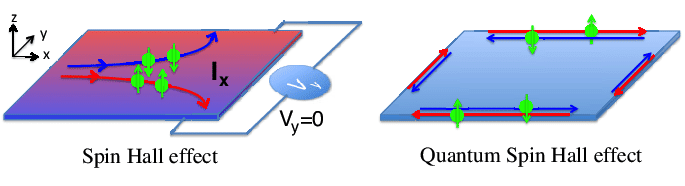
\includegraphics[width=\textwidth]{Immagini/ValleyHall/spin-hall-temp.png}
        \caption{In nonmagnetic conductor, equivalent currents in both spin channels with opposite ”anomalous velocity” leads to balanced electron concentration at both sides while net spin current in transversal direction. This leads to opposite moving spin edge states. Image taken from \cite{weng2015anomalous}.}
        \label{fig:gaps-topo-haldane}
    \end{figure}

